\chapter{Interaction modes}
\minitoc  

 \section{Object selection and what color is currently displayed? }
One very important aspect of MorphoDig's design is that most interactions or modifications of opened objects can only be done when these objects are selected. 
Selected objects (3D surfaces and landmarks) are always ``grey". All currently opened objects can be selected by pressing CTRL+A. All currently opened objects can be unselected by pressing CTRL+D. Objects can also be selected/unselected using the right mouse button, depending on the currently active interaction mode (see below). A given unselected surface can be colored: 

\begin{itemize}
\item using a uniform ``solid" color. Scalar display mode must be deactivated or active array combo box set to ``Solid color" (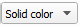
\includegraphics[scale=0.5]{images/04/scalarcombo_solidcolor.png})
\item according to the tag values (= integers) associated to the vertices. Array display mode button must be pressed (
\includegraphics[scale=0.7]{images/04/show_color_scale.png}), and a Tag array must be selected (ex:
\includegraphics[scale=0.5]{images/04/scalarcombo_tag.png}).
\item	according to the scalar values (= numbers) associated at the vertices. Array display mode button must be pressed (
\includegraphics[scale=0.7]{images/04/show_color_scale.png}), and a Scalar array must be selected (ex:
\includegraphics[scale=0.5]{images/04/scalarcombo_scalar.png})
\item	according to RGB values associated to the vertices. Array display mode button must be pressed (
\includegraphics[scale=0.7]{images/04/show_color_scale.png}), and a RGB array must be selected (ex:
\includegraphics[scale=0.5]{images/04/scalarcombo_rgb.png}) 
\end{itemize}





\section{Interaction modes}


\subsection{Camera mode}
  
\includegraphics[scale=0.7]{images/04/camera_mode.png}``Camera mode" is the default interaction mode, and is active on startup. When active, left and middle mouse button drags result in camera rotation/translation, respectively. Right mouse button drag results in object selection/unselection. Pressing "ESC" switches between object mode and camera mode.
\subsection{Object mode}
   
\includegraphics[scale=0.7]{images/04/move_mode.png}When active, left and middle mouse button drags result in object rotation/translation, respectively. Right mouse button drag results in object selection/unselection. Pressing "ESC" switches between object mode and camera mode.
\subsection{Landmark mode}
  
\includegraphics[scale=0.7]{images/04/Landmarks2.png}When active, only landmarks can be selected/unselected via right mouse button drag. This mode is useful when editing/placing landmarks. Left and middle mouse button drags result in camera rotation/translation, respectively.

\section{Landmark setting modes}
Landmarks can be set on surfaces by pressing ``L" + left mouse click. 
Four series of landmarks can be set with MorphoDig: ``normal" landmarks, ``target" landmarks, ``curve node" landmarks and ``curve handle" landmarks. Additionally a fourth special landmark series (``flag" landmarks) can be used to label surface structures. 

\subsection{Normal landmark mode}	
Press ``
\includegraphics[scale=0.7]{images/04/normal_landmarks.png}" to activate this mode (this mode is active by default)

\subsection{Target landmark mode}	
Press ``
\includegraphics[scale=0.7]{images/04/target_landmarks.png}"  to activate this mode

\subsection{Curve node mode}	
Press ``
\includegraphics[scale=0.7]{images/04/curve_nodes.png}" to activate this mode 

\subsection{Curve handle mode}	
Press ``
\includegraphics[scale=0.7]{images/04/curve_handles.png}"  to activate this mode


\subsection{Flag landmark mode}	
Press ``
\includegraphics[scale=0.7]{images/04/flag_landmarks.png}" to activate this mode
